\documentclass[conference]{IEEEtran}
\IEEEoverridecommandlockouts
\usepackage{cite}
\usepackage{amsmath,amssymb,amsfonts}
\usepackage{algorithmic}
\usepackage{graphicx}
\usepackage{textcomp}
\usepackage{xcolor}
\usepackage{multirow}
\def\BibTeX{{\rm B\kern-.05em{\sc i\kern-.025em b}\kern-.08em
    T\kern-.1667em\lower.7ex\hbox{E}\kern-.125emX}}
\begin{document}

\title{How to Know What You Don't Know: Open Set Deep Learning\\}

\author{\IEEEauthorblockN{Jordan Spell}
\IEEEauthorblockA{jdspell@iu.edu}
\and
\IEEEauthorblockN{Josiah Keime}
\IEEEauthorblockA{keimej@iu.edu}
\and
\IEEEauthorblockN{Kyle Firestone}
\IEEEauthorblockA{kfiresto@iu.edu}
}

\maketitle

\begin{abstract}
In this project we aim to explore image classification with open set deep learning networks, that is to say networks which are presented with image classes not contained in the training set and are tasked with being able to identify that these are unknown classes as opposed to confidently predicting these images belong to classes in the training set. We will further explore if these models cluster distinct unknown classes sufficiently different from each other that they can perform few-shot learning on the unknown classes. 
\end{abstract}

\section{Introduction}
Deep learning networks have immensely improved image classification over the past decade with numerous models achieving over 90\% top-1 accuracy on the ImageNet data set [1]. However, for many of these models they lack generalization and can struggle to perform in real-world scenarios where there are certainly more classes than the model was exposed to in its training set. For example, in autonomous driving it is unlikely that we could label every class a vehicle is likely to encounter. So, how then, does a  model behave when exposed to an image class that was not in the original data set? In some cases the model will incorrectly make a confident prediction of a class that was in the training set [2]. Even if there is no confident prediction, unless a prediction threshold rule has been put in place for the model, an incorrect class will still be predicted. This is the problem with closed set classification, the model assumes everything is a member of the training set classes. Open set models on the other hand are built with the knowledge that a model will see classes not in the training set and will train it to recognize that it does not know what class an image is.\\

Open set models were first considered outside of deep learning just as the deep learning revolution was taking place [3]. This approach utilized an SVM to determine how far was to far from a classification boundary and considered those as unknown classes. Since then several deep learning models have been developed looking at open set learning [4, 5]. The aim of this project is to explore existing open set deep learning frameworks and investigate improving these models. Specifically we will look at high dimensional embeddings of features learned from a network and use clustering in this embedded space to determine if an example is an unknown class. Furthermore, we aim to see if these models are capable of performing few-shot learning on these unknowns.

\section{Data Set Creation}

The data set used comes from Kaggle [6] and is composed of an internet image scrape of publicly available images of a variety of wildlife found throughout the Pacific Northwest. The data set consists of 14,013 images divided into 20 classes that are approximately class balanced. Due to the nature of the data set collection, manual pruning of the data set was conducted to remove anomalous images within the data set leaving a total of 12,375 images. For constructing the open set data of known and unknown classes, 15 classes were chosen to be known classes and the remaining 5 classes would be unknowns. The known classes were split into a train/validation/test split with a ratio of 70\%/15\%/15\% respectively while the unknowns were split into a validation/test split at a ratio of 20\%/80\%. The unknowns were chosen so as to provide a range of difficulty for the model to identify as an unknown class. For example, the unknown class of "columbian black-tailed deer" will likely be difficult to distinguish as an unknown since "deer" is in the known classes, but the unknown class "black bear" will likely be easier due to the lack of a similar class in the known data set.

\section{Baseline Models}

To determine if the choice of convolutional neural network would have an impact on the the ability to determine unknowns we chose to examine 3 different network architectures, namely ResNet, VGG19 and EfficientNetb0. The models were chosen so that each took the same image input size of $224 \times 224$ and had been pretrained with the ImageNet data set so had likely learned a diverse set of features during initial training that will transfer well to our specific data set. Transfer learning and fine-tuning were then applied to each model using the known data set. The specifics of each model are detailed below. All models were trained in TensorFlow V2.

\subsection{ResNet}

To train the ResNet model to our data set the pre-trained model was fed into a new head consisting of a global average pooling 2D layer, a batch normalization layer, a dropout layer and a final 15 node dense layer to perform the classification. Transfer learning was first applied by freezing the model weights of the ResNet layer and training with a learning rate of 0.001 with the Adam optimizer and categorical cross entropy loss function until model convergence as determined via early stopping. The model was then fine-tuned by unfreezing all the layer weights for the model and lowering the learning rate to $1e^{-5}$. Final top-1 accuracy on the validation set was 96\%.

\subsection{VGG19}

Transfer learning on VGG19 was performed similarly, with the original classification head being removed and replaced with a 15 node dense layer for our specific known class data set. For the initial transfer learning process only the new classification head was trained using the RMSProp optimizer with a learning rate of 0.001 and the categorical cross entropy loss function. Fine-tuning was performed by training all layer weights using the RMSProp optimizer with a learning rate of $1e^{-4}$ and the categorical cross entropy loss function. The model was able to achieve a final top-1 accuracy of 94\%.

\subsection{EfficientNetb0}

Lastly, transfer learning was applied to EfficientNetb0. The original classification head of the model was removed and replaced with a 15 node dense layer. All model weights with the exception of the new classification head were frozen and training was conducted over 100 epochs with a learning rate of 0.001 using the Adam optimizer and the categorical cross entropy loss function. This was followed with fine-tuning by unfreezing all model weights and reducing the learning rate to $1e^{-4}$ and training for an additional 50 epochs. After fine-tuning the model had a 95\% top-1 accuracy.

\section{Open Set Learning}

After fine-tuning, the open set learning process was started. We began by creating the additional model architecture necessary for learning the prototypes along with adding the loss functions required to learn the prototype features. This was followed by creating a distance-based triplet thresholding metric using the learned prototypes which the model uses to detect an image as an unknown class. Finally, few-shot learning on unknown classes is attempted.

\subsection{Prototype Learning}

In order to detect an image as unknown we project images into a higher dimensional feature space and identify unknowns based on the distance from representative examples of known classes in the feature space. This representative example is known as a prototype of a class. The idea of prototypes can be traced back to KNN and K-means clustering machine learning algorithms and would require hand crafted features. Yang, HM \textit{et. al.} [7] were the first to describe prototypes with deep learning models. The combination of open set and prototype learning was explored by Shu Y. \textit{et. al.} [5] and is the approach we follow for this project. We begin by creating a custom prototype layer for our pretrained models with a learnable zero-initialized weight matrix of dimension $15 \times 15$. The choice of dimension was chosen based on known classes, but there is no apriori reason the dimension of the feature space must match the number of known classes. In general, the prototype matrix can be of size $N \times M$ were $N$ is the number of classes and $M$ is the dimension of the feature space. In order to learn each class prototype we use 2 loss functions, one to learn the prototypes in feature space and a second to encourage proper classification and prevent prototypes from being overly influenced by outliers of a particular class. The first loss function to learn the protoypes is a squared $L_2$ loss defined by (1) where $B$ is the batch size, $f_i$ are the CNN extracted features of the $i^{\text{th}}$ image in the batch and $p_i$ is the prototype corresponding to the models' prediction for the $i^{\text{th}}$ image in the batch.

\begin{equation}
\mathcal{L}_1 = -\frac{1}{B} \sum_{i = 1}^B ||f_i - p_i ||_2^2
\end{equation}

For the second loss function we begin by creating an inverse distance distribution matrix, $D$, defined by

\begin{equation}
D_{i,j} = \frac{1}{|| f_i - p_j ||_2^2 + \epsilon}.
\end{equation}

This yields a $B \times 15$ matrix. The second prototype loss function is then given by (3) where $y_i$ is the ground truth OHE label for the $i^{\text{th}}$ image in the batch, $\sigma$ is the softmax function and $\cdot$ is the dot product operation.

\begin{equation}
\mathcal{L}_2 = -\frac{1}{B}\sum_{i = 1}^B \bigg( y_i \cdot \log \big( \sigma(D_{i, :}) \big) \bigg)
\end{equation}

The total loss function for learning the prototypes is given by $\mathcal{L}_{\text{prototype}} = \mathcal{L}_1 + \mathcal{L}_2$.\\

In addition to learning the protoypes we also want to promote the features of images to cluster as tightly to the prototypes as possible so it is easier to identify unknown classes once they are projected into the feature space. We accomplish this by learning a radius for each prototype that tries to minimize the distance each image falls from its corresponding prototype in feature space. A second zero-initialized trainable custom layer of dimension $1 \times 15$, one for each prototype, is created to learn the radii for each prototype. The loss function to learn these radii is then given by

\begin{equation}
\mathcal{L}_{\text{radii}} = -\frac{1}{C}\sum_{i = 1}^C \big( r_i - d_i \big)^2
\end{equation}

where $C$ is the number of correctly classified images, $r_i$ is the corresponding class radius of the $i^{\text{th}}$ correctly classified sample and $d_i$ is the maximum value of the corresponding row in $D$.\\

The total loss function for training the model then is given by (5) where $\mathcal{L}_{\text{CCE}}$ is the categorical cross entropy loss used to train the original classification models.

\begin{equation}
\mathcal{L} = \mathcal{L}_{\text{CCE}} + \alpha \mathcal{L}_{\text{prototype}} + \beta \mathcal{L}_{\text{radii}}
\end{equation}


\subsection{Triplet Thresholding}

For unknown detection we follow the approach by Shu, Y. \textit{et. al.} [8] which learns threshold values based on the distance distribution defined in (2). Specifically, the thresholds are a per-class triplet threshold ([$\eta_i$, $\mu_i$, $\delta_i$]) consisting of confidence acceptance threshold ($\eta$), confidence rejection threshold ($\mu$) and a distance rejection threshold ($\delta$) to make a classification or detect an unknown. These thresholds are given below where $F_{i, j}$ is the highest confidence value of the $i^{\text{th}}$ class of the $j^{\text{th}}$ correctly classified image as determined by $D$, $S_{i, j}$ is the second highest confidence value, $\mathcal{C}_i$ is the number of correctly classified images of class $i$ and $\gamma$ and $\rho$ are hyperparameters.

\begin{equation}
\eta_i = \frac{1}{\mathcal{C}_i} \sum_{j = 1}^{\mathcal{C}_i} F_{i, j}
\end{equation}

\begin{equation}
\mu_i = \gamma \eta_i
\end{equation}

\begin{equation}
\delta_i = \rho \frac{1}{\mathcal{C}_i} \sum_{j = 1}^{\mathcal{C}_i} \bigg( F_{i, j} - S_{i, j} \bigg)
\end{equation}

The acceptance threshold of an image is passed and classified as class $i$ when its highest confidence is of class $i$ and is above $\eta_i$ while an image is classified as an unknown when all confidence values are lower than $\mu$. When confidence values fall between $\eta$ and $\mu$ then $\delta$ is used and if the distance between the highest confidence class and the second highest confidence class is greater than $\delta$ then the image is assigned class $i$.

\subsection{Few-shot Learning}

In order to learn new classes the model encounters we take an incremental learning process outlined in [5]. We start by initializing a new prototype model that adds an extra class to the classification head, the prototype learning layer, the prototype radii layer and the triplet thresholds. When the model first encounters a new class, the weights of the new prototype are initialized as described in (9) where $N$ is the current number of classes and $\phi = (\phi_1, \phi_2, \cdots, \phi_N)$ are the normalized distance distributions.
\begin{equation}
w_{N+1} = \frac{1}{N}  \sum_{n = 1}^N \phi_n w_n
\end{equation}

After the first encounter of a new class, the model is trained as usual for what was previously an unknown class. When an additional novel class is added, the model size is updated as described above and the new weight is initialized as in (9).

\section{Experiments}

While we were unable to accomplish all of our goals for this model we did explore several different experiments. Firstly, we examined whether the prototype model was even learning by looking at the loss of the model during training. Secondly, we were interested in how the prototypes were evolving over training epochs so we tracked a single prototype over the entire training process and visualized the results with a low dimensional projection of the prototype. Next, we examined how well each known class is clustering during the course of training. For triplet thresholding we explored how the thresholds are updating each epoch. Finally, we conclude by looking at the clustering of known vs unknown classes to see if we are observing good separation between the two. 

\section{Results}

The efficacy of the prototype learning model to learn prototypes was validated by training the EfficientNetb0 model with the prototype modifications for 100 epochs using the known training data set with a learning rate of $1e^{-4}$ using the Adam optimizer and the combined loss function defined in (5). Figure 1 shows the results of this training, while the model seems to be performing well, the prototypes have not quite converged so perhaps further training would yield better results.\\

\begin{figure}
\centerline{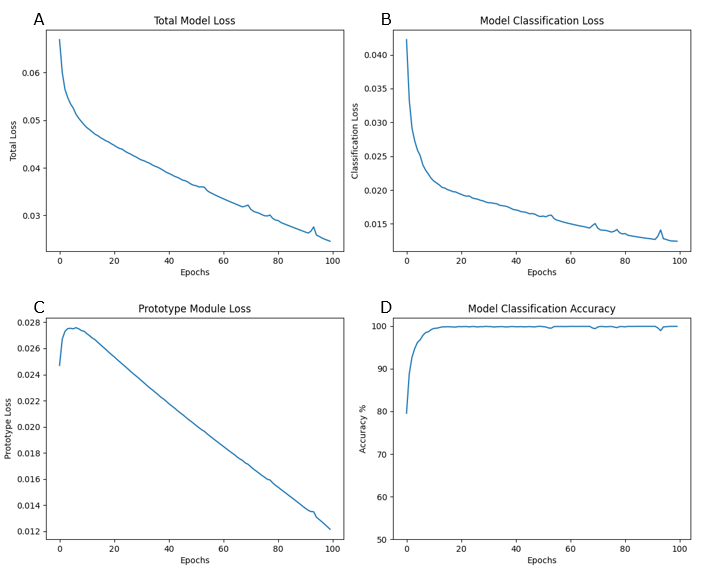
\includegraphics[scale=0.5]{Images/EffNet_Prototype_Training.png}}
\caption{Training the EfficientNetb0 prototype model. (A) Total model loss. (B) Classification loss. (C) Prototype and radii loss. (D) Model classification accuracy}
\label{fig}
\end{figure}

Figure 2 shows the ability of the ResNet model to learn a specific class prototype over training epochs visualized in 3-dimensional space using PCA dimensionality reduction. The model begins with large movements of the prototype trying to find the optimal position in feature space while towards the end of the 100 epoch training the prototype stabilizes to a more optimal position.\\

\begin{figure}
\centerline{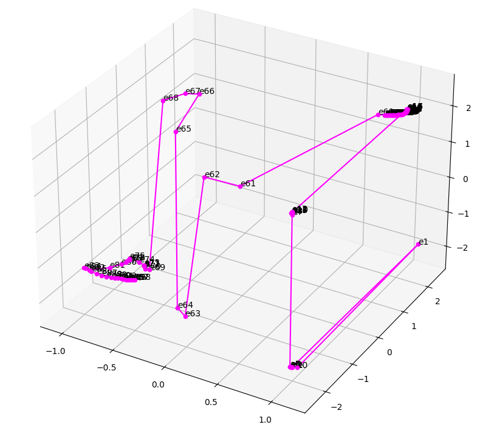
\includegraphics[scale=0.4]{Images/Prototype_Learning_Over_Epochs.png}}
\caption{Bobcat class prototype learning over 100 epochs in the ResNet model.}
\label{fig}
\end{figure}

To determine how well the model was learning good features that promoted tight clustering of classes in feature space we logged the output features of the training set for each known class in the ResNet model. Figure 3 shows these features for epochs 0, 10, 20 and 100 projected into 3-dimensional space using PCA reduction. We clearly see a positive impact of class clustering density during training.\\

\begin{figure}
\centerline{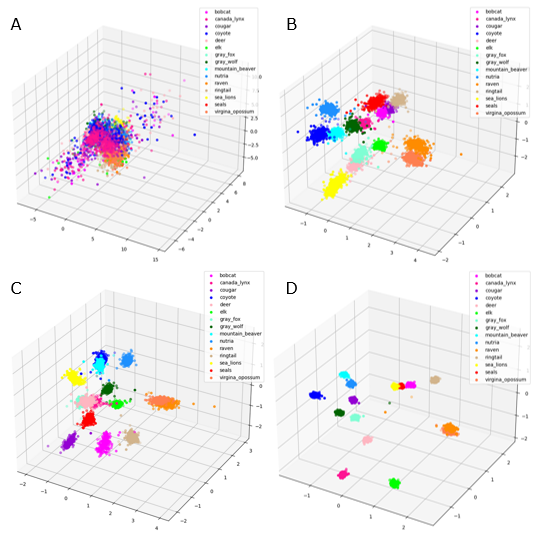
\includegraphics[scale=0.5]{Images/Image_Clusters_Over_Epochs.png}}
\caption{Clustering of validation images at different epochs in the ResNet model. (A) Epoch 0. (B) Epoch 10. (C) Epoch 20. (D) Epoch 100.}
\label{fig}
\end{figure}

We next looked at how the triplet thresholding for classification was changing during training. Figure 4 shows the results of the acceptance ($\eta$) and distance ($\delta$) thresholds during the prototype learning of ResNet for 100 epochs. We see a fairly monotonic increase in the thresholds over the training epochs which is presumably due to the model trying to be as generous as possible to classify the images. While using this new classification technique we were able to achieve a 93.3\% accuracy of known classes (3\% lower than softmax based classification), the ability to detect unknowns was extremely poor with only a 2.24\% detection rate. It is not immediately clear what the issue is and further study of the model would be required to diagnosis the issue.\\

\begin{figure}
\centerline{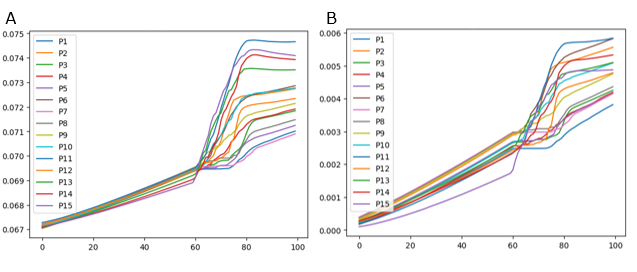
\includegraphics[scale=0.5]{Images/Thresholds_Over_Epochs.png}}
\caption{Classification triplet thresholds over 100 epochs for the ResNet model. (A) Acceptance threshold. (B) Distance threshold.}
\label{fig}
\end{figure}

Due to the poor ability of the triplet thresholding to detect unknown classes we wanted to know if poor clustering and seperation of the unknown classes relative to the knowns was a source of the poor performance. Figure 5 shows the clustering of unknown classes in blue and known classes in orange. The unknown classes are fairly diffuse, but do not seem to be overlapping with any of the plotted known classes. It could be that this poor clustering of unknown classes is contributing to the triplet thresholds inability to correctly identify unknowns and could be symptomatic of the models' features overfitting to the known classes.

 \begin{figure}
\centerline{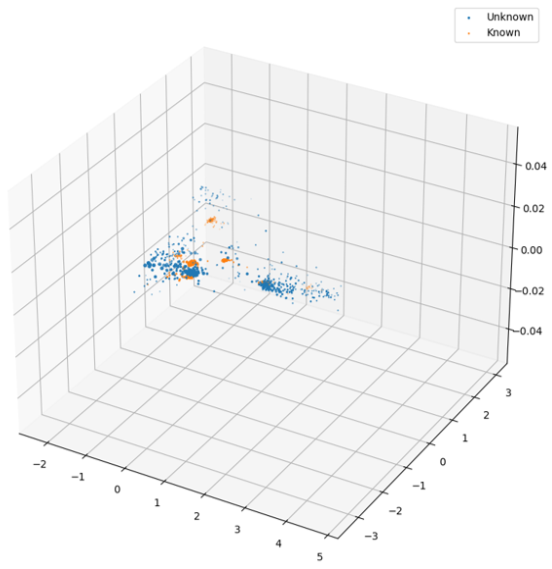
\includegraphics[scale=0.4]{Images/Known_vs_Unknown_Clustering.png}}
\caption{Clustering of known classes and unknown classes. Known classes in orange, unknown classes in blue.}
\label{fig}
\end{figure}

\section{Conclusion}

Here we present a method for creating a model that can recognize when it encounters images of classes it was not initially trained on by extracting features from a non-specialized convolutional neural network, learning features that when projected into feature space result in tightly grouped and separated clusters in the feature space to which a thresholding based classification system can be used. While we are able to achieve a high classification accuracy on known images, the ability of the model to recognize unknown images at present remains poor. Future work on this model would be to diagnosis the models poor ability to detect unknowns followed by getting the model to recognize unknowns with a few-shot learning technique.

\section{Supplemental}

All code for this project can be found at https://github.iu.edu/kfiresto/E533\_Final\_Project

\begin{thebibliography}{00}
\bibitem{b1} Papers with Code - ImageNet Benchmark (Image Classification) –- paperswithcode.com.

\bibitem{b2} A. Nguyen, J. Yosinski, and J. Clune. (2015) Deep neural networks are easily fooled: High confidence predictions for unrecognizable images. In Computer Vision and Pattern Recognition (CVPR), 2015 IEEE Conference on. IEEE.

\bibitem{b3} Scheirer, W., Rezende Rocha, A., Sapkota, A., \& Boult, T. (2013). Toward Open Set Recognition. IEEE Transactions on Pattern Analysis and Machine Intelligence, 35(7), 1757-1772.

\bibitem{b4} A. Bendale, \& T. E. Boult (2016). Towards Open Set Deep Networks. In 2016 IEEE Conference on Computer Vision and Pattern Recognition (CVPR) (pp. 1563-1572). IEEE Computer Society.

\bibitem{b5} Shu, Y., Shi, Y., Wang, Y., Huang, T., \& Tain, Y. (2020). “P-ODN: Prototype-Based Open Deep Network for Open Set Recognition.” Scientific Reports, vol. 10, no. 1,  p. 7146.

\bibitem{b6} Molina, D. (2019). Oregon wildlife. Retrieved from https://www.kaggle.com/datasets/virtualdvid/oregon-wildlife

\bibitem{b7} Hong-Ming Yang, Xu-Yao Zhang, Fei Yin, \& Cheng-Lin Liu (2018). Robust Classification with Convolutional Prototype Learning. CoRR, abs/1805.03438.

\bibitem{b8} Yu Shu, Yemin Shi, Yaowei Wang, Yixiong Zou, Qingsheng Yuan, \& Yonghong Tian (2019). ODN: Opening the Deep Network for Open-set Action Recognition. CoRR, abs/1901.07757.

\end{thebibliography}

\end{document}
